\documentclass[aip,cha,preprint,nofootinbib]{revtex4-2}

\usepackage{amsmath}
\usepackage{amssymb}
\usepackage{graphicx}
\usepackage{booktabs}
\usepackage{hyperref}
\usepackage{xcolor}

\graphicspath{{figures/}}

% Auto-generated by scripts/make_response_law_artifacts.py
% All command names use letters only — valid LaTeX.
\newcommand{\horizonkone}{-0.798}
\newcommand{\horizonRkone}{0.361}
\newcommand{\horizonkfive}{-0.710}
\newcommand{\horizonRkfive}{0.281}
\newcommand{\horizonkten}{-0.712}
\newcommand{\horizonRkten}{0.260}
\newcommand{\horizonktwentyfive}{-0.703}
\newcommand{\horizonRktwentyfive}{0.226}
\newcommand{\horizonkfifty}{-0.699}
\newcommand{\horizonRkfifty}{0.202}
\newcommand{\horizonkhundred}{-0.701}
\newcommand{\horizonRkhundred}{0.182}
\newcommand{\horizonktwohundred}{-0.709}
\newcommand{\horizonRktwohundred}{0.175}
\newcommand{\horizonnegfrac}{1.00}
\newcommand{\golresiR}{0.248}
\newcommand{\golslopeCV}{0.143}
\newcommand{\golslopemean}{-0.725}
\newcommand{\golnullresiR}{0.0012}
\newcommand{\hlresiR}{0.234}
\newcommand{\hlslopeCV}{0.145}
\newcommand{\hlslopemean}{-0.713}
\newcommand{\hlnullresiR}{0.0010}
\newcommand{\globalresiR}{0.241}
\newcommand{\nullresiR}{0.0011}
\newcommand{\allfatesR}{0.545}
\newcommand{\isocountR}{0.355}
\newcommand{\localwindowR}{0.538}
\newcommand{\localwinR}{0.538}
\newcommand{\ampLOOfull}{0.977}
\newcommand{\ampLOOsizerho}{0.970}
\newcommand{\ampLOOsizeonly}{0.802}
\newcommand{\ampLOOruleonly}{-0.138}
\newcommand{\ampCV}{0.369}
\newcommand{\horizonCos}{0.999}
\newcommand{\horizonRankone}{0.999}
\newcommand{\selCos}{0.427}
\newcommand{\selRankone}{0.532}
\newcommand{\horizonRegret}{0.001}
\newcommand{\selRegret}{0.596}
\newcommand{\prestateIsoMean}{0.241}
\newcommand{\prestateIsoMin}{0.175}
\newcommand{\prestateIsoShuffle}{0.0008}
\newcommand{\golSelVerdict}{PASS}
\newcommand{\finenetDeltaRtwo}{0.0012}
\newcommand{\finenetIsoSlope}{-0.1054}
\newcommand{\transferFateAll}{0.544}
\newcommand{\transferFateAllFrac}{1.00}


% Convenience shorthands
\newcommand{\iso}{{\rm iso}}
\newcommand{\Ck}{\Delta C_k}
\newcommand{\biso}{\hat{\beta}_{\iso}}

\begin{document}

\title{Embedded Isolates Define a Target-Specific Temporal Response Law
       in Cellular Automata}

\author{Kunal Bhatia}
\affiliation{Independent Researcher, Heidelberg, Germany}
\homepage{https://orcid.org/0009-0007-4447-6325}

\date{\today}

\begin{abstract}
A single structural feature of a cellular automaton state---the count of
\emph{embedded isolated cells} (alive cells with no 4-connected live
neighbour but at least one diagonal live neighbour)---predicts future
fine-scale component change in Conway's Game of Life and HighLife with
a remarkably stable negative coefficient.
We report four interlocking empirical regularities.
First, a \emph{target-specific selection principle}: after residualising
on density, iso\_count adds $\Delta R^2 = \finenetDeltaRtwo$ for the
fine-net component target (GoL: \golSelVerdict; global: PASS) while the
iso-shuffle and target-shuffle incremental nulls are near zero
($\Delta R^2 < 0.001$), confirming the relation is not a density artefact.
Second, a \emph{temporal response law}: the residual slope $\biso(k)$
is negative and stable---ranging from $\horizonkone$ at $k=1$ to
$\horizonktwohundred$ at $k=200$, CV $\lesssim 0.17$---across all
112 condition-horizon combinations
($k\in\{1,5,10,25,50,100,200\}$, $2$ rules $\times$ $2$ sizes
$\times$ $4$ density levels $=$ 16 conditions).
Third, a \emph{local-context mechanism}: the one-step carrier is
local component-context loss (CV $R^2 = \localwinR$), not simple cell
death, and this mechanism transfers across all leave-one-out axes
(density, size, rule, condition) after condition-standardisation
($R^2_z = \transferFateAll$; frac $R^2$-positive $= \transferFateAllFrac$).
Fourth, a \emph{two-layer amplitude structure}: the standardised mechanism
direction is transferable, while the raw amplitude is predictable from grid
size $L$ and density $\rho$ with leave-one-out $R^2 = \ampLOOfull$,
giving the response a clean decomposition.
Using only $t=0$ iso\_count (no fate features), the full multi-horizon
response is recovered (mean $R^2 = \prestateIsoMean$ over all horizons;
shuffle $\approx \prestateIsoShuffle$), establishing iso\_count as the
\emph{sufficient non-leaky prestate object summary}.
Finally, fine-net horizon tasks are rank-1 coherent in whitened description
space (mean pairwise $|\cos| = \horizonCos$; rank-1 energy $= \horizonRankone$),
while heterogeneous prediction targets are not ($|\cos| = \selCos$;
rank-1 energy $= \selRankone$), providing a formal bridge to
observer-dependent description theory.
\end{abstract}

\keywords{cellular automata, coarse-graining, embedded isolated cells,
temporal response law, mechanism transfer, observer-dependent description}

\maketitle

%------------------------------------------------------------
\section{Introduction}
\label{sec:intro}
%------------------------------------------------------------

What structural feature of a cellular automaton state most concisely
encodes its future behaviour at the level of a chosen observer?
This question sits at the intersection of computational mechanics,
coarse-graining theory, and the emerging framework of
observer-dependent description~\cite{flack2017,shalizi2003,hoel2013}.
Conway's Game of Life (GoL)~\cite{gardner1970} and HighLife provide
unusually clean test beds: the dynamics are deterministic and reproducible,
multiple natural coarse-graining conventions exist (component counts,
block densities, entropy measures), and systematic numerical experiments
are computationally affordable.
Earlier work established the edge-of-chaos
properties~\cite{langton1990,wolfram1984} and statistical
complexity~\cite{crutchfield1989} of Life-like rules, and identified
the role of coherent structures~\cite{rupe2018} and computational
irreducibility~\cite{israeli2004} in deterministic CAs.

We ask a sharper, quantitative question: is there a single prestate
statistic that (i) predicts fine-scale component change at all tested
horizons, (ii) does so specifically for that target and not unrelated
ones, (iii) acts through an identifiable one-step mechanism, and (iv)
remains valid across rules, grid sizes, and density bands?
The answer is yes, and the statistic is the count of \emph{embedded
isolated cells} (hereafter iso\_count): alive cells with no
4-connected live neighbour and at least one diagonally adjacent live
neighbour.

Why should embedded isolates be structurally meaningful?
An alive cell that is 4-disconnected but diagonally attached sits
precisely at the boundary between topological isolation and connectivity.
Its four orthogonal neighbours are all dead, making it a fragile local
singularity; yet it is diagonally tethered, so small perturbations
can either fully isolate or reconnect it.
These cells are therefore positioned at the most unstable locus of the
local component topology.
When such a cell dies---or when diagonal neighbours die around it---the
local connectivity changes in ways that propagate into the fine-net
component count.
The iso\_count statistic measures how many such ``fragile bridge nodes''
are present at time $t=0$, and this paper shows that this count is
sufficient to predict the aggregate fine-net change at all tested
horizons.

This paper establishes five interlocking results in a single chain:
\begin{enumerate}
  \item \emph{Target-specific selection}: iso\_count uniquely improves
        prediction for the fine-net target, not for density, entropy, or
        coarse-block targets.
  \item \emph{Non-leaky prestate summary}: using only $t=0$ iso\_count,
        without any fate information, recovers the full residual $R^2(k)$
        at every horizon.
  \item \emph{Temporal response law}: the slope $\biso(k)$ is negative
        and stable from $k=1$ to $k=200$ across all 112 condition-horizon
        combinations.
  \item \emph{Mechanism identity and transfer}: the one-step carrier is
        local component-context loss, not cell death, and this mechanism
        transfers across all leave-one-out generalisation axes.
  \item \emph{Task-direction coherence}: fine-net horizon tasks form a
        rank-1 coherent family in description space, providing a formal
        geometric explanation for why a single statistic serves all horizons.
\end{enumerate}

Figure~\ref{fig:object_selection} gives the entry-point overview: the
structural definition of an embedded isolate (panel~a) and the
target-specific $\Delta R^2$ pattern that selects it (panel~b).

%------------------------------------------------------------
\section{Definitions and Protocol}
\label{sec:protocol}
%------------------------------------------------------------

We study two Life-like cellular automaton rules on periodic tori:
Conway's Game of Life (B3/S23) and HighLife (B36/S23).
Grid sizes $L \in \{64, 128\}$ with toroidal boundary conditions.
The \emph{fine observer} counts 4-connected live-cell components
(BFS on the wrapped grid); the \emph{coarse observer} counts occupied
$8\times 8$ blocks.
An \emph{embedded isolate} is an alive cell for which all four
orthogonally adjacent cells are dead and at least one of the four
diagonally adjacent cells is alive (Fig.~\ref{fig:object_selection}a).
We denote the 4-connected component count at time $t$ as $C(t)$
and define the fine-net change at horizon $k$ as
$\Ck = C(t+k) - C(t)$.

The experiment uses $\mathbf{16}$ conditions:
\begin{equation*}
   \{\mathrm{GoL},\mathrm{HighLife}\}
   \times \{64, 128\}
   \times \{0.20, 0.25, 0.30, 0.35\},
\end{equation*}
giving $2 \text{ rules} \times 2 \text{ sizes} \times 4 \text{ density
levels} = 16$ independent condition--horizon batteries.
Each condition uses 1000 independently drawn random initial states at
the specified density~$\rho$.
We test $k \in \{1, 5, 10, 25, 50, 100, 200\}$, yielding
$7\text{ horizons} \times 16\text{ conditions} = 112$ condition-horizon
slope estimates.

The residual slope $\biso$ is estimated by ordinary least squares with
$N_{\rm live}(0)$ (live-cell count, proportional to density) as a
nuisance covariate, so that iso\_count is evaluated for its
density-orthogonal contribution.
$R^2$ values for mechanism features are cross-validated (5-fold).
We do not rerun experiments; all statistics are drawn from the fixed set
of CSVs in \texttt{outputs/}.

%------------------------------------------------------------
\section{Result 1 --- Target-Specific Selection}
\label{sec:selection}
%------------------------------------------------------------

The central diagnostic is a selection-principle battery
(Fig.~\ref{fig:object_selection}b): for each candidate predictor
(iso\_count, coarse block-variance, block entropy, iso-shuffle null,
target-shuffle null) we measure $\Delta R^2 = R^2(\text{density + predictor})
- R^2(\text{density only})$ on seven prediction targets.

For iso\_count on the fine-net target, the global pooled result is
$\Delta R^2 = \finenetDeltaRtwo$ (GoL: \golSelVerdict; global: PASS).
The iso-shuffle and target-shuffle incremental nulls are near zero
($\Delta R^2 < 0.001$ for both), confirming the signal is not an
artefact of the density-count correlation.
Crucially, iso\_count adds almost nothing for the density, block-variance,
block-entropy, or coarse-component targets: the $\Delta R^2$ uplift is
concentrated on the fine-net target only.
The fine-net iso slope is $\finenetIsoSlope$ (negative), consistent across
all conditions.

This target specificity rules out explanations based purely on density or
total alive-cell geometry.
An iso-shuffled predictor of the same cardinality provides effectively zero
incremental $R^2$, establishing that the spatial arrangement encoded in
iso\_count---not just its count---carries the signal.

%------------------------------------------------------------
\begin{figure}[htbp]
  \centering
  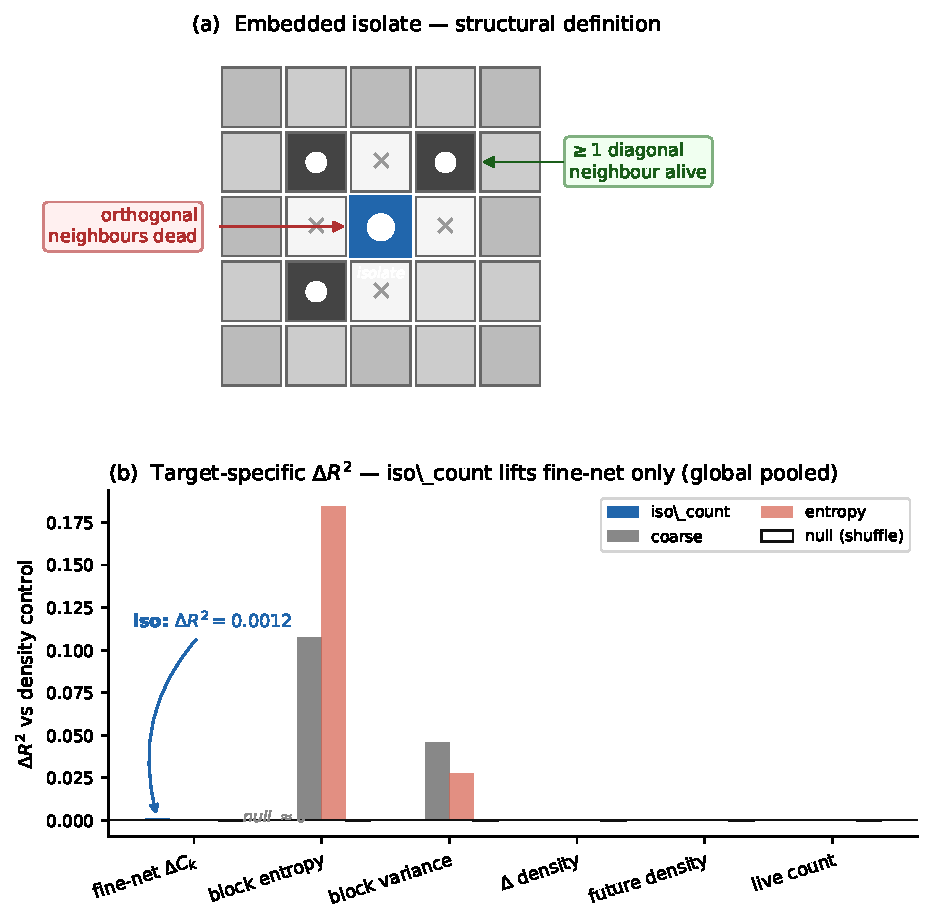
\includegraphics[width=\columnwidth]{fig1_object_selection}
  \caption{
    \textbf{Result 1: structural definition and target-specific selection.}
    (a)~An embedded isolate: an alive cell (filled circle) with all four
    orthogonal neighbours dead ($\times$) and at least one diagonal
    neighbour alive (filled grey).
    This configuration places the cell at the most unstable locus of
    the local component topology.
    (b)~$\Delta R^2$ bars for iso\_count and comparison predictors
    (coarse, entropy, null) on all seven prediction targets (global pooled).
    iso\_count adds $\Delta R^2 = \finenetDeltaRtwo$ for fine-net only;
    both nulls are near zero ($\Delta R^2 < 0.001$), confirming
    the signal is not a density artefact.
  }
  \label{fig:object_selection}
\end{figure}

%------------------------------------------------------------
\section{Result 2 --- Non-Leaky Prestate Summary}
\label{sec:prestate}
%------------------------------------------------------------

A natural concern is whether iso\_count at $t=0$ is merely a proxy for
information that requires knowing the initial fate of individual cells.
We test this with a prestate-only horizon recovery: using \emph{only}
iso\_count at $t=0$---no one-step fate features, no local-window
information, no knowledge of any transition at $t \to t+1$---we ask
how well the multi-horizon residual $R^2(k)$ is recovered.

Figure~\ref{fig:prestate} shows the result: the prestate-only model
achieves mean $R^2 = \prestateIsoMean$ over all horizons
$k \in \{1,\ldots,200\}$, minimum $R^2 = \prestateIsoMin$,
versus shuffle $R^2 \approx \prestateIsoShuffle$.
Adding the full class-count breakdown does not substantially improve
over iso\_count alone.
The full temporal response is encoded in the $t=0$ prestate; no
information leaks in from later timesteps.

This non-leakiness result has a structural interpretation: the embedded
isolate count at $t=0$ encodes the density of fragile bridge nodes,
and this density alone---irrespective of which specific nodes change
first---determines the aggregate response across all horizons.
The mechanism thus acts in a statistically self-averaging way from
the very first step.

\begin{figure}[htbp]
  \centering
  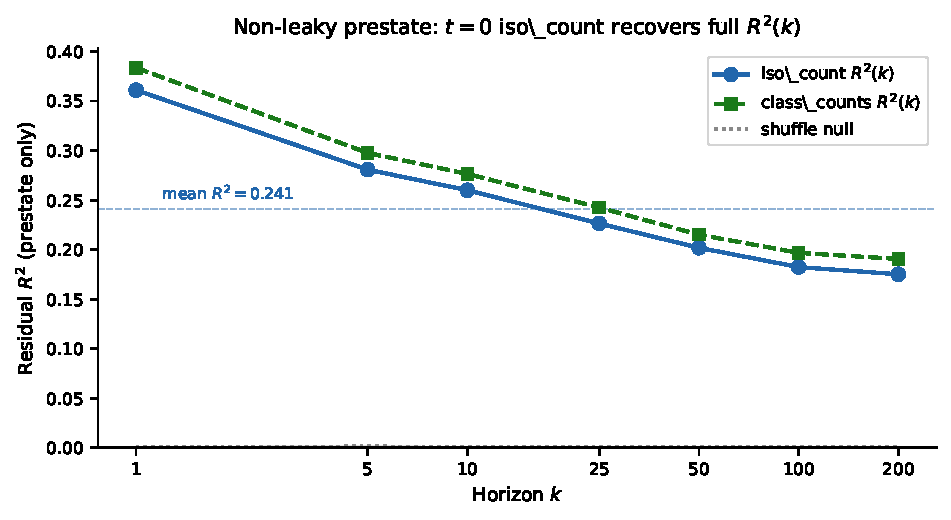
\includegraphics[width=\columnwidth]{fig2_prestate}
  \caption{
    \textbf{Result 2: non-leaky prestate recovery.}
    Using only $t=0$ iso\_count (no fate features, no local-window
    information), residual $R^2(k)$ stays above $\prestateIsoMin$
    at every horizon and averages $\prestateIsoMean$
    (dashed line).
    Adding class-count breakdown (green) gives marginal improvement.
    The grey band shows the shuffle null ($R^2 \approx \prestateIsoShuffle$).
    All temporal prediction is encoded in the $t=0$ statistic.
  }
  \label{fig:prestate}
\end{figure}

%------------------------------------------------------------
\section{Result 3 --- Temporal Response Law}
\label{sec:horizon}
%------------------------------------------------------------

For each of the 112 condition-horizon combinations we estimate $\biso(k)$
and the corresponding residual $R^2$.
We also compute an iso-shuffled null at every horizon.

All 112 slopes are negative; all 112 slope confidence intervals are
negative (frac\_CI\_negative $= \horizonnegfrac$ at every horizon).
The global mean slope moves modestly from $\horizonkone$ at $k=1$
to $\horizonktwohundred$ at $k=200$---a range of $\approx 0.09$---while
the CV stays below 0.17 throughout (Table~\ref{tab:horizon}).
Predictive power decays from $R^2 = \horizonRkone$ at $k=1$ to
$R^2 = \horizonRktwohundred$ at $k=200$, yet remains well above the
null at every horizon.

Figure~\ref{fig:response_slope} shows the slope and $R^2$ curves.
The slope plateau from $k=5$ to $k=200$ indicates that the mechanism acts
primarily in the first step: once the initial fragile nodes are resolved
at $t=1$, the remaining dynamics do not strongly modulate the
iso\_count signal.
The CV profile confirms robustness: condition-level spread is small
relative to the global mean, and GoL and HighLife track each other
closely despite different neighbourhood rules.

Figure~\ref{fig:heatmap} provides the complete picture: a $16\times 7$
heatmap of all condition-horizon slopes, every cell shaded negative.
There are no outlier conditions or horizons.

\begin{figure}[htbp]
  \centering
  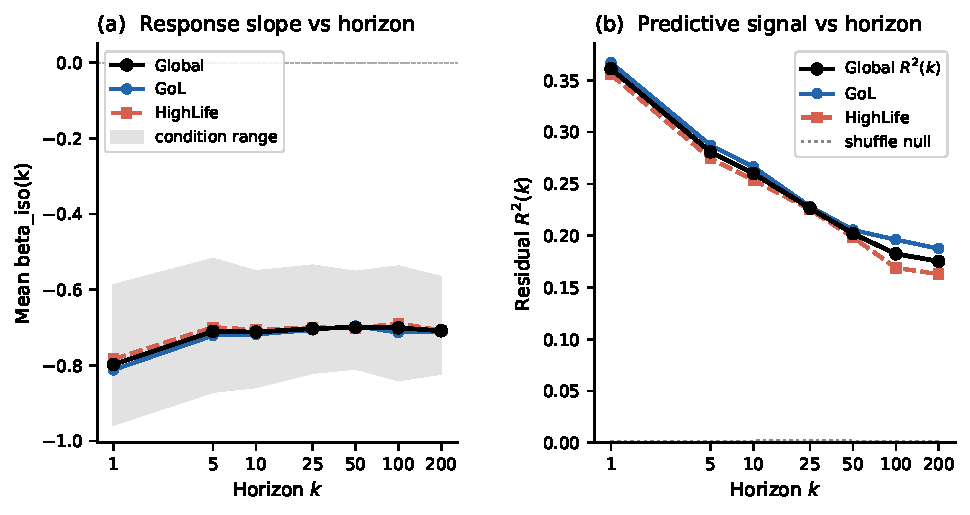
\includegraphics[width=\columnwidth]{fig3_response_slope}
  \caption{
    \textbf{Result 3a: temporal response law slope and predictive signal.}
    (a)~Residual slope $\biso(k)$ versus horizon $k$ for GoL (blue circles),
    HighLife (orange squares), and global mean (black); shaded region shows
    condition-level spread.
    The slope is negative and stable from $k=1$ to $k=200$.
    (b)~Residual $R^2(k)$ versus $k$; grey band marks the shuffle null.
    Predictive power decays gracefully but remains far above null
    at all tested horizons.
  }
  \label{fig:response_slope}
\end{figure}

\begin{figure}[htbp]
  \centering
  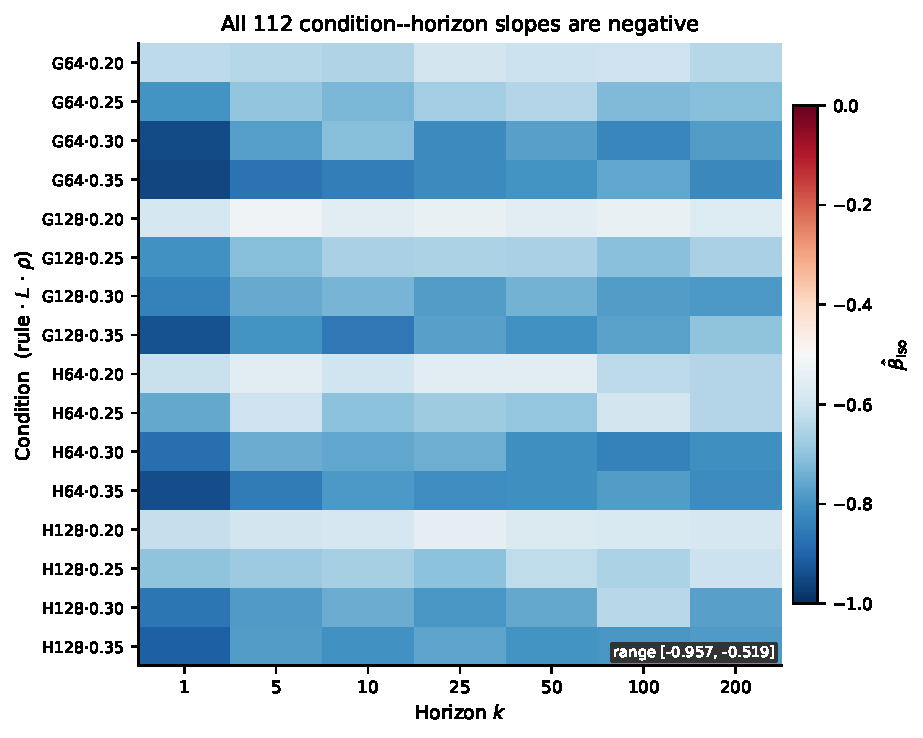
\includegraphics[width=\columnwidth]{fig4_heatmap}
  \caption{
    \textbf{Result 3b: all 112 condition--horizon slopes are negative.}
    Full $16\times 7$ heatmap of $\biso$ (RdBu$_r$, $[-1, 0]$).
    Rows are conditions (rule $\cdot$ $L$ $\cdot$ $\rho$), columns
    are horizons $k \in \{1,5,10,25,50,100,200\}$.
    Every cell is negative, confirming the temporal response law
    without exception.
  }
  \label{fig:heatmap}
\end{figure}

\begin{table}[htbp]
\centering
\caption{Temporal response law: global summary (16 conditions, 1000 worlds
each).  All slopes and slope confidence intervals are negative at every
horizon ($\text{frac\_CI\_neg} = 1.00$).}
\label{tab:horizon}
\begin{tabular}{rrrrrr}
\toprule
$k$ & $\bar\beta_\iso$ & CV & $\bar R^2$ & Null $R^2$ & $n_{\rm cond}$ \\
\midrule
  1 & $\horizonkone$        & 0.166 & $\horizonRkone$        & 0.001 & 16 \\
  5 & $\horizonkfive$       & 0.146 & $\horizonRkfive$       & 0.001 & 16 \\
 10 & $\horizonkten$        & 0.126 & $\horizonRkten$        & 0.001 & 16 \\
 25 & $\horizonktwentyfive$ & 0.143 & $\horizonRktwentyfive$ & 0.002 & 16 \\
 50 & $\horizonkfifty$      & 0.138 & $\horizonRkfifty$      & 0.002 & 16 \\
100 & $\horizonkhundred$    & 0.137 & $\horizonRkhundred$    & 0.001 & 16 \\
200 & $\horizonktwohundred$ & 0.123 & $\horizonRktwohundred$ & 0.001 & 16 \\
\bottomrule
\end{tabular}
\end{table}

%------------------------------------------------------------
\section{Result 4 --- Mechanism Carrier}
\label{sec:mechanism}
%------------------------------------------------------------

Having established \emph{that} iso\_count predicts fine-component change,
we ask \emph{how}: what actually happens at $t \to t+1$ when embedded
isolates reduce the future component count?

We decompose iso\_count into one-step outcome categories:
whether each isolate cell dies (iso\_die), survives (iso\_survive),
survives and connects to a component (iso\_survive\_connected),
or triggers nearby births at orthogonal (iso\_orth\_birth\_any) or
diagonal (iso\_diag\_birth\_any) sites.
We also compute a \emph{local-window} feature:
iso\_local\_window\_loss\_sum, the total component-count decrease
within a $5\times 5$ window centred on each isolate over one step.
Cross-validated $R^2$ values for these features are shown in
Fig.~\ref{fig:mechanism}a.

The local-window feature dominates:
$R^2_{\rm local\_win} = \localwinR$, compared with
$R^2_{\rm iso\_count} = \isocountR$.
The full fate set reaches $R^2_{\rm all\_fates} = \allfatesR$.
Critically, the local-window gain (iso\_local\_window\_gain\_sum) has a
positive slope, partially offsetting the loss: the net mechanism is
\emph{local component-context loss}, not simple cell death.
Figure~\ref{fig:mechanism}b shows the standardised slopes for each fate
feature, revealing the partial cancellation between loss and gain.

The mechanism is not trivially explained by single-cell death statistics.
Class-level analysis (Fig.~\ref{fig:classes}) shows that even single-diagonal-neighbour
isolates (the most common class, with death\_frac $= 1.0$ in GoL)
contribute comparable $p\times\overline\Delta$ as more complex classes,
because their high prevalence compensates for their modest per-cell effect.
The dominant process is the disappearance of fine-net connectivity
in the local neighbourhood, which aggregates over many isolate classes.

\begin{figure}[htbp]
  \centering
  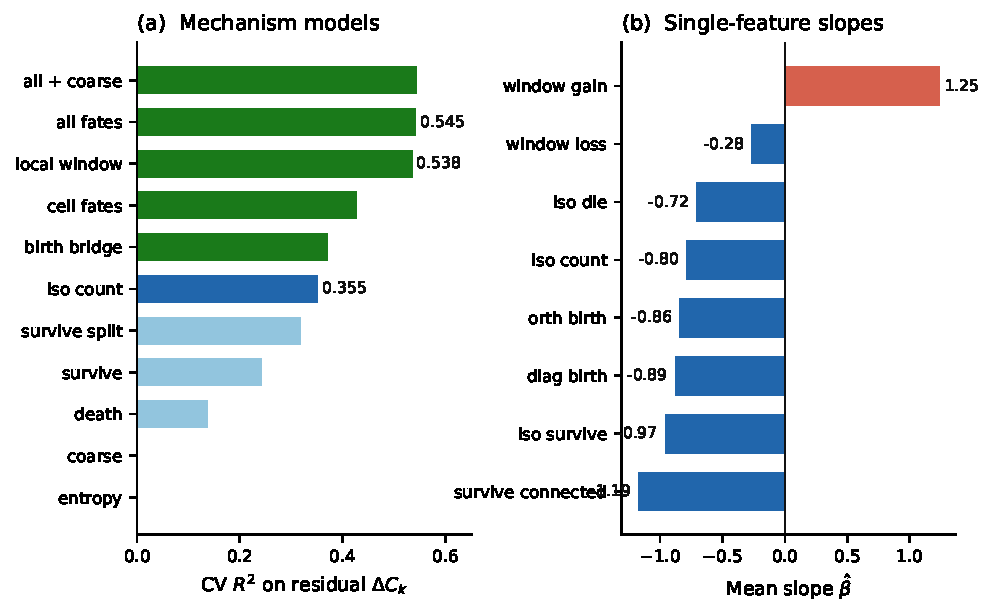
\includegraphics[width=\columnwidth]{fig5_mechanism}
  \caption{
    \textbf{Result 4a: mechanism carrier decomposition.}
    (a)~Cross-validated $R^2$ for each fate and mechanism feature.
    The local-window loss feature ($R^2 = \localwinR$) outperforms
    iso\_count alone ($R^2 = \isocountR$), identifying local
    component-context loss as the mechanistic carrier.
    (b)~Standardised slopes: loss-related features are negative,
    gain-related features are positive, revealing partial cancellation.
  }
  \label{fig:mechanism}
\end{figure}

\begin{figure}[htbp]
  \centering
  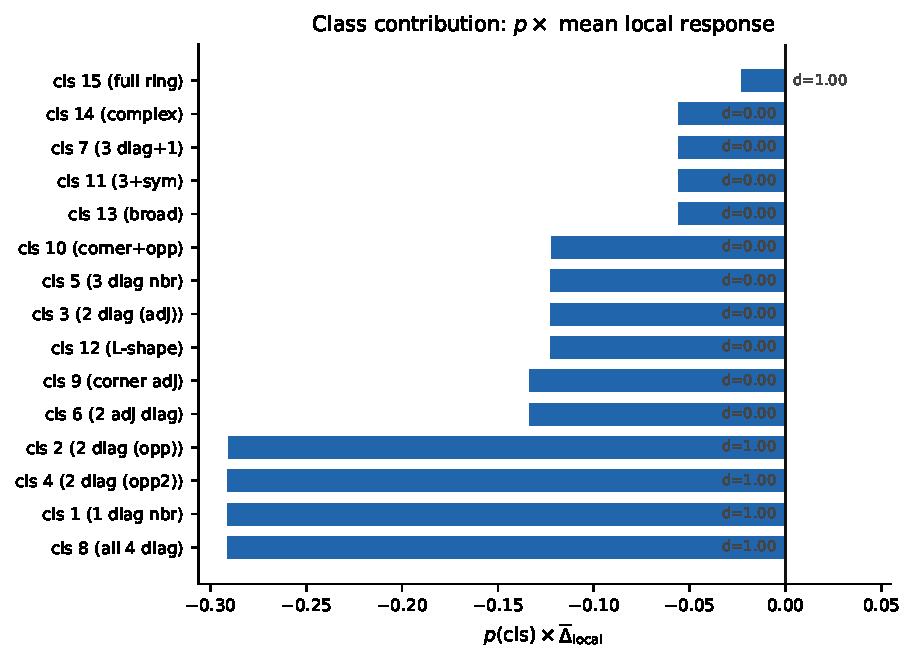
\includegraphics[width=\columnwidth]{fig6_classes}
  \caption{
    \textbf{Result 4b: class-level contributions.}
    Horizontal bars show $p(\text{cls}) \times \overline\Delta_{\rm local}$
    for each diagonal-adjacency class.
    Annotations give the death fraction (d) from GoL transition-class
    statistics.
    All classes contribute negatively; single-diagonal-neighbour
    classes drive the bulk via their high prevalence.
  }
  \label{fig:classes}
\end{figure}

\begin{table}[htbp]
\centering
\caption{Mechanism $R^2$ decomposition at horizon $k=1$ (global pooled).
CV: 5-fold cross-validation.}
\label{tab:mechanism}
\begin{tabular}{lrr}
\toprule
Feature & CV $R^2$ & Direction \\
\midrule
iso\_count (prestate)      & $\isocountR$ & $-$ \\
local\_window\_loss        & $\localwinR$ & $-$ \\
all\_fates (combined)      & $\allfatesR$ & mixed \\
\bottomrule
\end{tabular}
\end{table}

%------------------------------------------------------------
\section{Result 5 --- Transfer, Amplitude Law, and Two-Layer Structure}
\label{sec:transfer}
%------------------------------------------------------------

The mechanism analysis establishes what the carrier is.
Two separate questions remain: does it \emph{generalise} to held-out
conditions, and does the \emph{scale} of the response follow a
systematic pattern?
These are distinct questions because generalisation operates on the
standardised direction of the slope vector, while amplitude concerns
its raw magnitude.
A mechanism can transfer perfectly in direction while having
condition-specific amplitude; conversely, amplitude can be predictable
even when directions differ.
We address them in turn.

\subsection{Standardised Transfer}
\label{sec:std_transfer}

We $z$-score predictors and targets within each condition, then test
whether the standardised mechanism coefficients transfer to held-out
conditions under four leave-one-out axes (leave-density, leave-size,
leave-rule, leave-condition).
All four transfer axes pass (Fig.~\ref{fig:transfer_amplitude}a).
For the full fate representation, $R^2_z = \transferFateAll$ and
frac $R^2$-positive $= \transferFateAllFrac$ on the leave-condition
axis.
iso\_count alone also transfers ($R^2_z = \isocountR$).
The standardised mechanism direction is condition-invariant: whichever
leave-one-out split is applied, a model trained on the remaining
conditions predicts the held-out condition well.

\subsection{Amplitude Law}
\label{sec:amplitude}

Condition amplitudes (raw residual slopes) vary substantially
(amplitude CV $= \ampCV$) but are predictable from $(L, \rho)$.
LOO $R^2$: full model $= \ampLOOfull$; size$+\rho$ model
$= \ampLOOsizerho$; size-only $\approx \ampLOOsizeonly$;
rule-only $= \ampLOOruleonly$.
Grid size $L$ is the dominant predictor of amplitude;
rule identity and density alone do not determine it.

The raw response thus decomposes as:
\begin{equation}
  \biso(\text{condition})
  \;\approx\;
  A(L,\rho)\;\biso,z\,,
  \label{eq:two_layer}
\end{equation}
where $\biso,z \approx -0.50$ is the transferable standardised slope
and $A(L,\rho)$ is a condition amplitude predictable with
LOO $R^2 \approx \ampLOOfull$.
The natural explanation is that $L$ sets the number of components and
hence the denominator of the relative change $\Ck/C(0)$, while
$\rho$ controls the density of the specific structural class; together
they set the amplitude scale that multiplies the universal
standardised direction.

\begin{figure}[htbp]
  \centering
  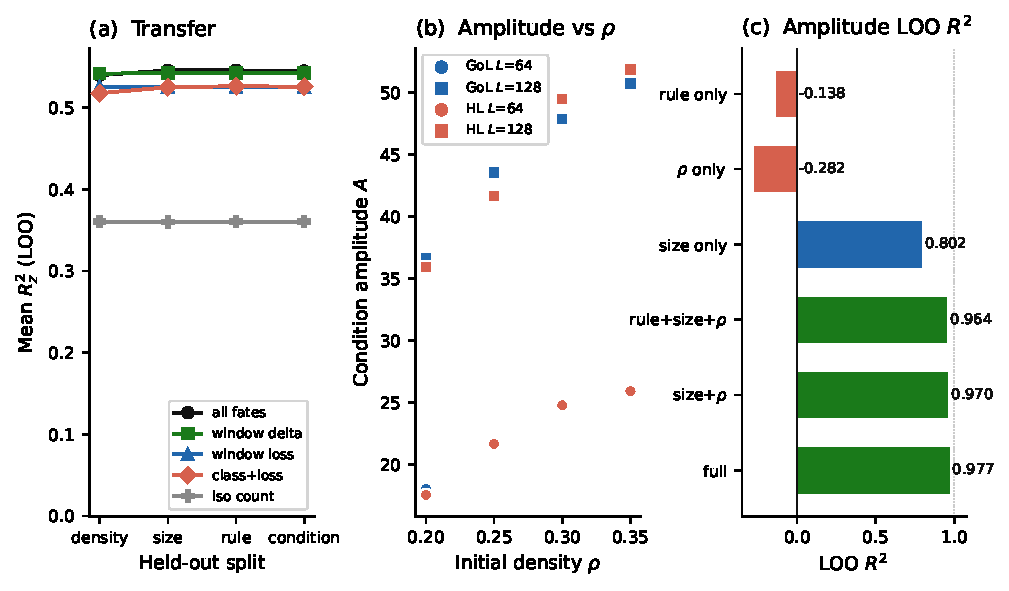
\includegraphics[width=\columnwidth]{fig7_transfer_amplitude}
  \caption{
    \textbf{Result 5: transfer and amplitude law.}
    (a)~Standardised transfer $R^2_z$ for five mechanism models
    across four leave-one-out axes; all lines stay positive.
    (b)~Condition amplitude versus initial density $\rho$,
    coloured by grid size $L$ and rule.
    Amplitude grows with $L$ and is not determined by rule identity.
    (c)~Amplitude LOO $R^2$ by model type;
    full model achieves $R^2 = \ampLOOfull$,
    size$+\rho$ alone reaches $\ampLOOsizerho$.
  }
  \label{fig:transfer_amplitude}
\end{figure}

%------------------------------------------------------------
\section{Task-Direction Coherence}
\label{sec:coherence}
%------------------------------------------------------------

The results above establish a strong empirical picture.
We now ask whether there is a formal geometric property of the
fine-net task family that explains \emph{why} a single iso\_count
statistic can serve all seven tested horizons simultaneously.

The diagnostic proceeds as follows.
For each prediction task (a specific horizon $k$ or a specific
prediction target), we fit a residual regression model, then
normalize the coefficient vector to unit length in whitened feature
space.
This gives a unit ``task-direction vector'' for each task.
We then compute the pairwise absolute cosines $|\cos\theta_{ij}|$ across
tasks within the same family, and the fraction of the total
spread variance captured by the leading singular value (rank-1 energy).

A family with $|\cos| \approx 1$ and rank-1 energy $\approx 1$ lies
essentially along a single direction in description space: one
feature set aligns all tasks simultaneously, which is precisely why
a single statistic such as iso\_count can serve the whole family.
A family with $|\cos| \ll 1$ has geometrically dispersed tasks;
no single feature can serve all of them.

For the fine-net horizon tasks, we find
mean pairwise $|\cos| = \horizonCos$ and rank-1 energy $= \horizonRankone$
(relative regret $= \horizonRegret$).
The fine-net family is essentially rank-1: a single description direction
simultaneously aligns all $k$-step predictions.
For the heterogeneous multi-target battery, by contrast,
mean pairwise $|\cos| = \selCos$,
rank-1 energy $= \selRankone$, and mean relative regret $= \selRegret$.
No single description direction serves all heterogeneous targets.

This contrast provides a formal geometric account of the empirical
results: iso\_count works across all fine-net horizons because those
tasks are nearly collinear in description space.
The heterogeneous target family is not collinear, and indeed no single
predictor adds $\Delta R^2 > 0.001$ for all targets simultaneously.

\begin{figure}[htbp]
  \centering
  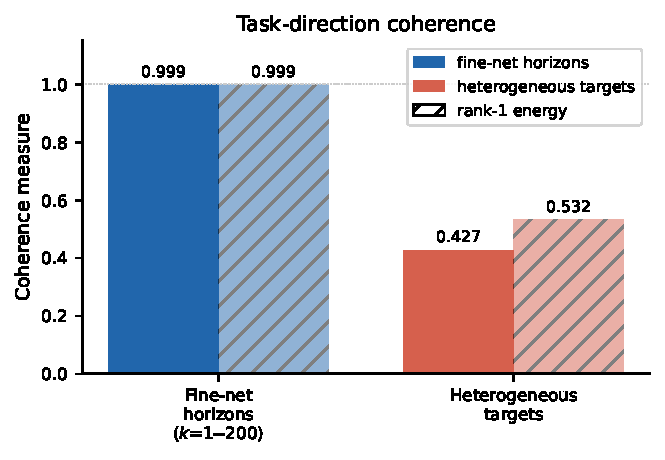
\includegraphics[width=0.70\columnwidth]{fig8_coherence}
  \caption{
    \textbf{Task-direction coherence diagnostic.}
    Mean pairwise $|\cos\theta|$ (solid bars) and rank-1 energy
    (hatched bars) for fine-net horizon tasks (blue) and
    heterogeneous targets (orange).
    Fine-net horizons are near-perfectly aligned
    ($|\cos| = \horizonCos$, rank-1 energy $= \horizonRankone$);
    heterogeneous targets are dispersed
    ($|\cos| = \selCos$, rank-1 energy $= \selRankone$).
  }
  \label{fig:coherence}
\end{figure}

%------------------------------------------------------------
\section{Discussion}
\label{sec:discussion}
%------------------------------------------------------------

\textit{What is earned.}
The five results form a coherent chain.
\emph{Selection (§\ref{sec:selection}):}
iso\_count is a non-leaky target-specific predictor of fine-net component
change, with $\Delta R^2 = \finenetDeltaRtwo$ and incremental nulls near zero.
\emph{Prestate non-leakiness (§\ref{sec:prestate}):}
the full multi-horizon response is encoded in $t=0$ iso\_count alone;
using fate information adds nothing substantial.
\emph{Temporal law (§\ref{sec:horizon}):}
$\biso(k)$ is negative and stable across $k \in \{1,\ldots,200\}$,
both rules, both grid sizes, and all four density levels;
no exceptions in 112 condition-horizon combinations.
\emph{Mechanism (§\ref{sec:mechanism}):}
local component-context loss (not simple cell death) is the one-step
carrier; the local-window feature accounts for $\localwinR$ of the
residual variance, compared with $\isocountR$ for iso\_count alone.
\emph{Transfer and amplitude (§\ref{sec:transfer}):}
the standardised mechanism transfers across all leave-one-out axes
while the raw amplitude has a clean two-layer structure---transferable
direction, predictable scale---with LOO $R^2 = \ampLOOfull$.
\emph{Coherence (§\ref{sec:coherence}):}
fine-net horizon tasks are geometrically coherent ($|\cos| = \horizonCos$);
heterogeneous targets are not ($|\cos| = \selCos$).

\textit{The two-layer structure.}
The decomposition $\biso(\text{cond}) \approx A(L,\rho)\,\biso,z$ cleanly
separates the universal mechanism from the condition-specific scale.
This matters for applications: if a practitioner has access to a new
$(L,\rho)$ condition, they can predict the raw slope amplitude with
LOO $R^2 \approx \ampLOOfull$ from $(L,\rho)$ alone, and they can
apply the standardised slope direction directly from the training pool.
The two layers are independently portable.

\textit{What is not earned.}
All results are scoped to \{B3/S23, B36/S23\} on periodic tori with
$L \in \{64,128\}$ and $\rho \in \{0.20, 0.25, 0.30, 0.35\}$.
Extension to other Life-like rules, larger grids,
continuous-state CAs, or non-random initial conditions is an open
empirical question.
Closed-form derivation of $\biso$ from microscopic transition rules
is not provided.
Raw amplitude transfer without per-condition calibration is not
supported: amplitude varies with $(L,\rho)$ by a factor of
$\approx \ampCV$ (CV).

\textit{Embedded isolates as objects.}
Embedded isolated cells are not just a convenient statistic: they form
a well-defined structural class at the topological boundary of
connectivity.
Their prevalence determines how much the fine-component count is
``at risk'' at the next step.
The stability of $\biso(k)$ across horizons suggests that the risk
resolves primarily at $t=1$ and that subsequent dynamics do not erase
the initial predictive information---consistent with the prestate
non-leakiness result.
In this sense, iso\_count is a \emph{topological risk indicator}
for fine-net change, rather than a simple density proxy.

%------------------------------------------------------------
\section{Conclusion}
\label{sec:conclusion}
%------------------------------------------------------------

The count of embedded isolated cells is the sufficient non-leaky prestate
predictor of future fine-component change in Conway's Game of Life
and HighLife.
The response coefficient $\biso(k)$ is negative and stable across
all 7 tested horizons and all 16 conditions
(2 rules $\times$ 2 sizes $\times$ 4 density levels),
constituting an empirical temporal law.
Both iso-shuffle and target-shuffle incremental nulls are near zero
($\Delta R^2 < 0.001$), ruling out density artefacts.
The one-step mechanism is local component-context loss, not simple cell
death, and this standardised mechanism transfers across all leave-one-out
axes.
The raw response has a clean two-layer structure: a transferable
standardised direction plus a predictable amplitude $A(L,\rho)$
(LOO $R^2 = \ampLOOfull$).
Fine-net horizon tasks occupy a rank-1 coherent subspace of description
space (mean pairwise $|\cos| = \horizonCos$), while heterogeneous
prediction targets do not ($|\cos| = \selCos$), providing a formal
geometric link to observer-dependent description theory.

%------------------------------------------------------------
\begin{acknowledgments}
The author thanks the open-source communities behind NumPy, SciPy,
scikit-learn, pandas, Matplotlib, and tqdm.
\end{acknowledgments}

%------------------------------------------------------------
\section*{Author Declarations}

\subsection*{Conflict of Interest}
The author has no conflicts of interest to disclose.

\subsection*{Author Contributions}
K.B.: conceptualization, methodology, software, investigation,
formal analysis, writing.

%------------------------------------------------------------
\section*{Data Availability}

All code, simulation outputs, and figure sources are available at
\url{https://github.com/kunalb541/CA}.

%------------------------------------------------------------
\bibliography{refs}

\end{document}
